\chapter{Background} \label{chap:sota-bg}

\section{Architecture of Traditional Optimizing Compilers}

Fully discussing the history of compiler construction is out of scope for this work. However, we present an overview of the architecture of modern compilers, taking as examples LLVM, GCC, and CompCert.

Modern, retargetable compilers emerged to solve the so-called \textit{$m \times n$ problem}: how can we reduce the work of providing a compilation infrastructure that support a set of source languages (such as C, C++, FORTRAN, Ada, Rust, and so on) and yet also be able to generate optimized code for several hardware architectures (such as x86 and x86-64, Arm, POWER, RISC-V, and so forth), while avoiding a combinatorial explosion of implementation effort?

\begin{figure}
    \centering
    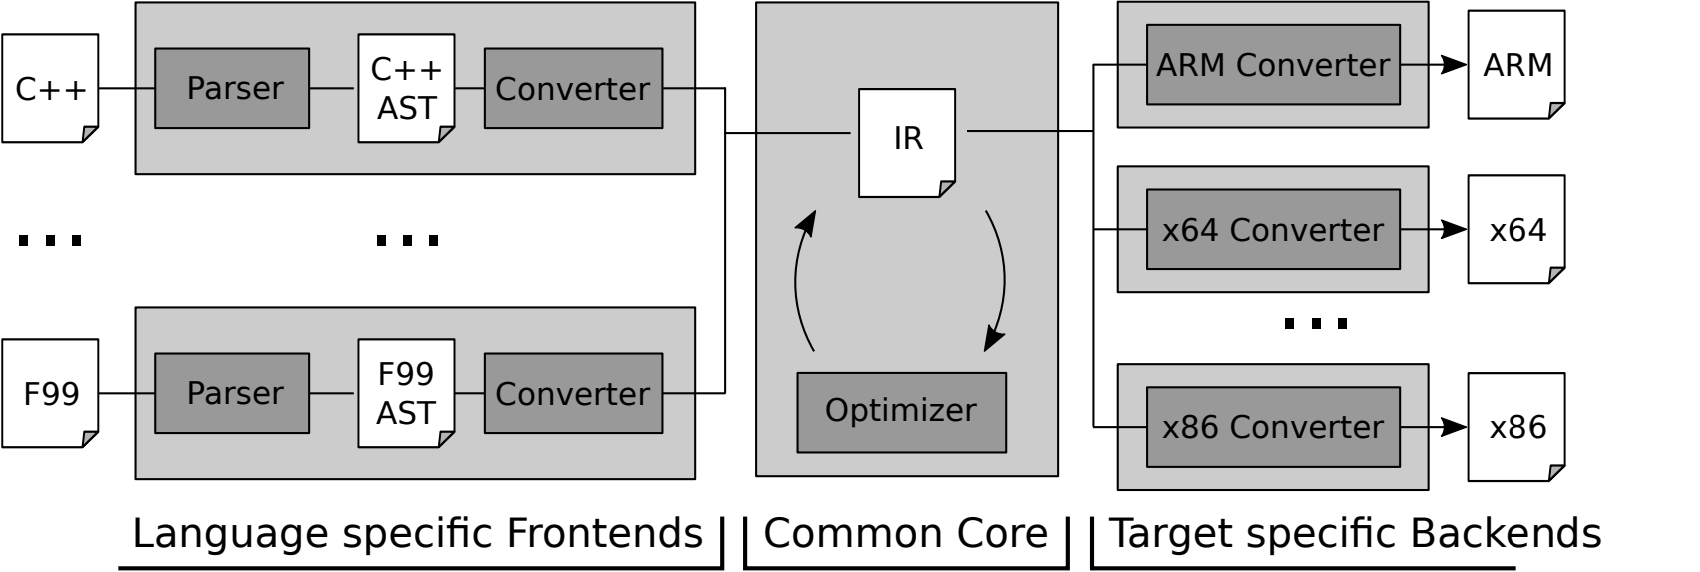
\includegraphics[width=\textwidth]{figures/generic_compiler_arch.png}
    \caption{A conceptual model of a retargetable compiler. Re-printed from \cite{Zangerl2018}}
    \label{fig:generic_compiler}
\end{figure}

To do so, they relied on two key insights: that these high-level languages were able to be transformed down to equivalent code in a subset of core imperative primitives that is still hardware-independent, and that this low-level intermediate representation (IR) contains enough information to perform most common optimizations.

Therefore, as seen in Figure~\ref{fig:generic_compiler}, we can conceptualize the retargetable compiler as a system consisting of three separate sets of modules:

\begin{itemize}
    \item Front-ends: these modules are responsible for parsing and checking the semantics of the source code, and then transforming it to the common intermediate language, which might imply compiling down language-specific features, such as monomorphization, dynamic dispatch, and so on. Usually, one front-end is implemented for each supported high-level language.
    \item Common core: this module is responsible for performing the bulk of the optimization steps, repeatedly transforming the program. Because these transformations are coded in terms of the intermediate representation, they can be re-used by each pair of source and target.
    \item Back-ends: Finally, the optimized code is processed to transform it to a code suitable for the final target, by performing target-specific tasks such as register allocation, instruction selection, linking according to the platform conventions, etc. These modules are usually implemented for each supported target.
\end{itemize}

Figure ~\ref{fig:llvm_arch} shows that LLVM's architecture aligns closely with this model. Support for each language or language family is implemented in separate front-ends (Clang for C/C++, rustc for Rust, the Julia compiler, etc.), which then generate code in the LLVM IR to be optimized by the LLVM optimizer, and finally a backend such as LLVM CodeGen \cite{LLVMCodeGen} can generate the output code (x86-64, Arm, WebAssembly), or another backend such as \textit{lli} \cite{LLVMDirectExecution} can directly interpret or JIT-compile the optimized IR.

\begin{figure}
    \centering
    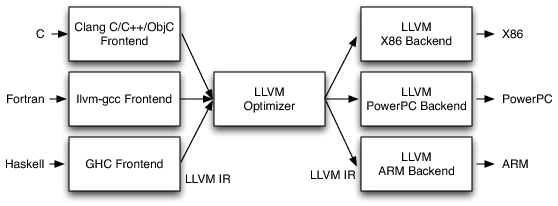
\includegraphics[width=\textwidth]{figures/llvm_arch.png}
    \caption{Diagram of LLVM compiler infrastructure's architecture. Reprinted from \cite{LattnerAOSA}}
    \label{fig:llvm_arch}
\end{figure}

Other compiler projects take a similar approach to their architecture. The GNU Compiler Collection uses several Intermediate Representations throughout the compilation process \cite{Novillo2004} - GENERIC, an abstract syntax tree representation; GIMPLE, a three-address-code representation; and a register transfer language - to simplify operations in different sections of the pipeline, and help modularize an otherwise monolithic architecture. Ongoing efforts \cite{GCCRearch} are being undertaken to further modularize this system into separate front-end, middle-end and back-end modules.
CompCert\cite{Leroy2009Compiler}, a formally verified compiler for the C programming language, also uses several intermediate representations to aid their goal of implementing and verifying each stage of the compilation process (see Figure ~\ref{fig:compcert_arch}).

\begin{figure}
    \centering
    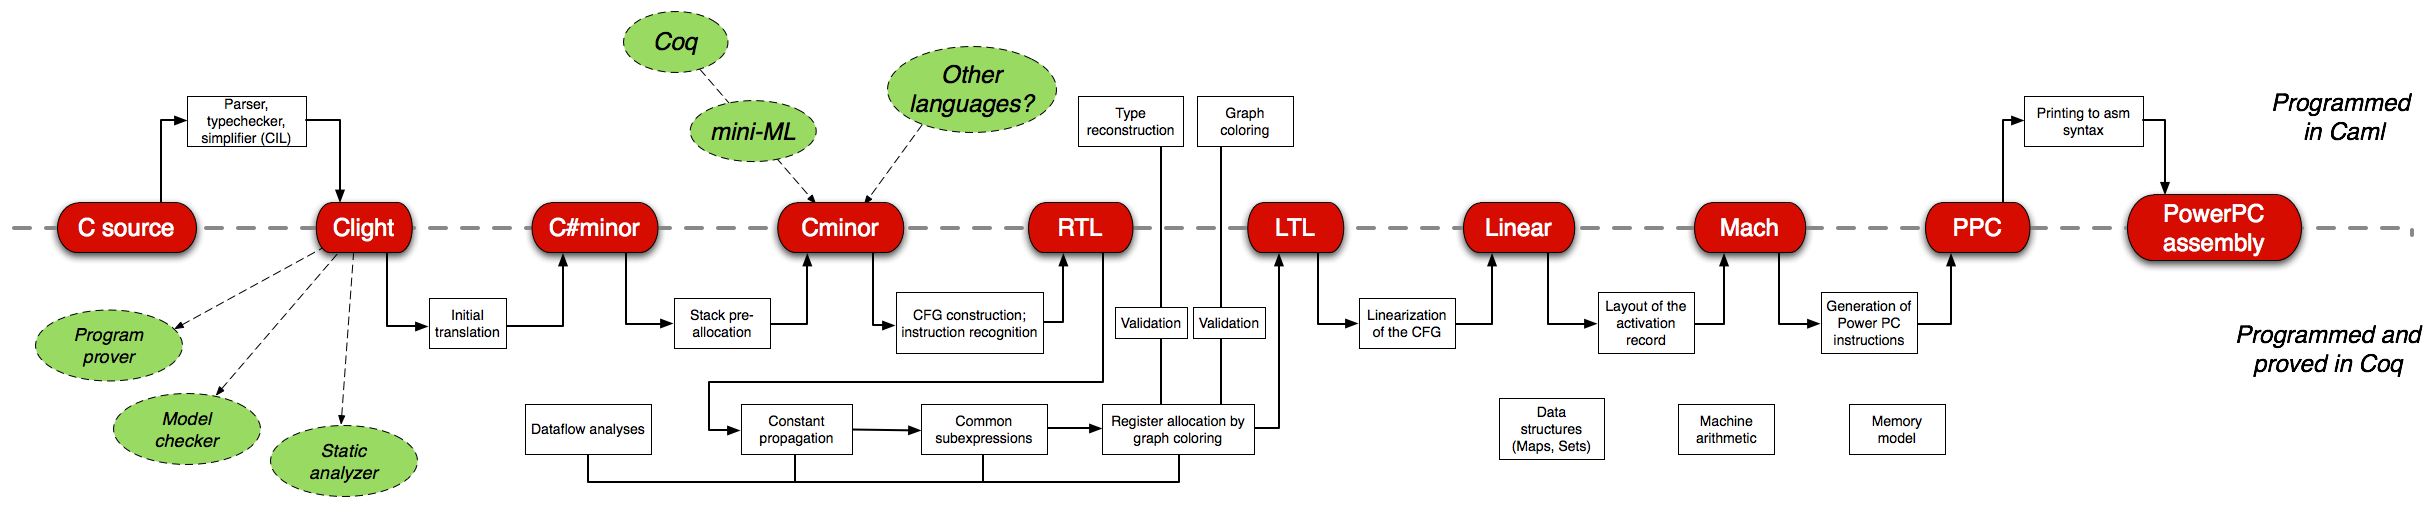
\includegraphics[width=\textwidth]{figures/compcert_arch.png}
    \caption{Diagram of CompCert's architecture. Reprinted from \cite{CompCertHome}}
    \label{fig:compcert_arch}
\end{figure}

\section{Optimization Techniques}

For the aims of our work, it proves useful to understand the kind of techniques that are commonly utilized to transform user-supplied codes into equivalent, yet more performant programs. This is done through analyzing the code and determining opportunities for transforming it into an optimized form, and performing those transformations, usually as a series of \textit{passes}, which yield a transformed version of the program.

We specifically wish to highlight two different aspects of the optimization process: the scope of the analyses, and the nature of the applied transformations.

\subsection{Scope of analysis for optimization}

Seeing as the first step of the optimization process is an analysis step, to determine which optimizations can be applied, we can distinguish optimizations by which scope the analysis is done.

The smallest scope is \textbf{local code analysis}. This analysis considers distinct instructions or small blocks of instructions. For example, let us consider the \textit{strength reduction} optimization. This optimization substitutes specific instances of complex instructions for equivalent but simpler, and therefore faster to execute, instructions. Consider the following two codes:

\begin{lstlisting}[language=C]
// prologue
// assume this variable exists and is set through an external interaction
int input_var;

// before strength reduction
int transformed_var = input_var * 4;

// after strength reduction
int transformed_var = input_var << 2;
\end{lstlisting}

The analysis is able to transform a multiplication by a power of two by an equivalent arithmetic shift instruction. Notice that, to perform this optimization, the analysis needs to just consider the one line of code, or a small block of instructions (load from memory, multiply with an immediate, store to memory). Therefore, it is \textit{local} in scope. In fact, this optimization can even be applied by linearly scanning the generated low-level code and replacing the instruction directly, in a process called \textit{peephole optimization}.

An intermediate scope at which analyses can be performed, and probably the most common one, is that of \textbf{global code analysis}\cite{Kildall1973}. This kind of analysis considers all visible code in a self-contained block, which usually corresponds to a function or procedure in the high-level language. Because such a scope might contain branching control and data-flow, stemming from the existence of loops and conditionals, these analyses rely on more advanced techniques, such as control and data-flow analysis\cite{Cytron1991}, logical induction of variables, etc, but in turn are able to deliver transformations that stem from the interaction between different blocks of instructions.

Some examples of this scope of analyses are:

\begin{itemize}
    \item Constant folding and propagation, or compile-time evaluation - this technique substitutes complex expressions whose arguments are only constants by the use of a single constant, that is yielded by performing the computation at the time of compilation.
    \item Common sub-expression elimination - this analysis detects expressions where a factor is repeatedly computed, and reworks the code to only compute it once, storing its value in a temporary variable to be reused.
    \item Loop unrolling - this analysis duplicates the body of a loop in the code, to perform fewer branches, which may improve instruction pipelining on the CPU.
    \item Dead code elimination - eliminates sections of the code which are unreachable, based on an analysis of the program's control flow.
    \item Some kinds of strength reduction, such as substituting the iterative computation of an arithmetic series by its direct computation, are only possible through global analyses, such as inductive variable analysis.
\end{itemize}

Even though this scope of analysis often suffices to perform many useful transformations, it carries the limitation that calls into other global scopes, such as calls to other functions, procedures, and units of compilation, are opaque, meaning that transformations which need information from several global scopes are impeded. To solve that issue, another scope of analysis is needed, \textbf{inter-procedural analysis}. On this scope, the interactions between different procedures are considered by analyses. Let us consider the following code as an example:

\begin{lstlisting}[language=C++]
template <type T>
class vector<T> {
    const T get(size_t i) const  {
        if (i < size) {
            return array[i];
        } else {
            throw Exception(/*...*/);
        }
    }

    size_t get_size() const {
        return size;
    }


    private:
    T* array;
    size_t size;
}

int main(void) {
    auto vec = new vector<int>();

    // initializing code here ...

    for (size_t i = 0; i < vec.get_size(); i++) {
        auto elem = vec.get(i);
        std::cout << elem * elem << '\n';
    }
}
\end{lstlisting}

In this code listing, we can intuit that there are several optimization opportunities that go unexploited unless we consider the interaction between both functions:

\begin{itemize}
    \item On line 26, a naïve call to the \textit{get\textunderscore{}size} function will involve multiple operations related to calling the function - saving to the stack a number of values whose registers might be overwritten, storing the parameters and the return instruction pointer in specific registers or stack positions, jumping to the subroutine, storing the return values in specific registers or stack positions, jumping back to the callee, restoring the values that were previously ejected from the registers, etc - even though the body of the function itself consists only of loading a number from a memory address. By using an inter-procedural analysis such as \textit{function inlining}, which duplicates the body of the called function inside the body of the caller, the compiler is able to remove such operations, yielding a simpler version of the code.
    \item While we can recognize that the loop header in line 26 and the branch in line 4 contain a duplicated condition check, simple global analysis in each procedure will not be able to detect such redundancy. However, an \textit{inter-procedural dead code elimination} analysis is able to do so, and remove the redundant check and associated unreachable code.
\end{itemize}

\subsection{Nature of transformations}

When considering which transformations can be applied in the context of optimizing codes, we distinguish the nature of the transformation, in relation to how it affects the performance of the code and the process of optimization itself.

Often, a transformation can itself be considered a \textbf{direct optimization}. The nature of these transformations is that they directly improve the performance of the transformed code. For example, strength reduction operations directly substitute computations for equivalent yet cheaper operations, directly improving the speed of the code. Likewise, constant propagation and folding allows computation to be shifted from run-time to compilation time, allowing expensive computations to be replaced by cheap loading of an immediate value.

On the other hand, some transformations might benefit the optimization process, regardless of their direct impact on the codes' performance. We term these \textbf{enabling transformations}. These transformations enable previously impossible optimizations, surfacing an emergent optimization property from the composition of different techniques\cite{Click1995}.

For example, function inlining may or may not impact positively the performance of the code\cite{Chen1993}, depending on the balance between the improved instruction pipelining, and the worsened program size, which may affect negatively the caching of the program's instructions. In any case, the extra information that the body of the inlined function provides may be instrumental in performing other analyses and transformations, such as dead code elimination, vectorization, or constant folding.

Another example of this phenomenon is constant folding and propagation. Besides directly reducing the amount of computation performed at run time, it may enable the compiler to prove that certain code paths are unreachable, aiding the process of dead code elimination.

Furthermore, some transformations, which are often called \textit{normalization} transformations, have the explicit goal of putting the analysed codes in a \textit{canonical form}, so that latter analyses have fewer edge cases to contend with, making the transformation code simpler and more maintainable. Examples of these include factoring complex computations into several temporary variables, or normalizing loop headers\cite{Gomes2021} e.g. so that they are always of the form \texttt{for (int i = 0; i < N; i++)}.

\section{Summary}

In this chapter, we have given an overview of important background concepts, for our work, namely by describing the three-stage architecture of modern optimizing compilers, and by categorizing the scope and nature of the analyses and transformations that they may perform on the programs they compile.